%-------------------------------------------------------------------------------
%	PACKAGES AND OTHER DOCUMENT CONFIGURATIONS
%-------------------------------------------------------------------------------

\documentclass{article}

% Packages
% Packages

% \usepackage{fancyhdr} % Required for custom headers
% \usepackage{lastpage} % Required to determine the last page for the footer
% \usepackage{extramarks} % Required for headers and footers
% \usepackage[usenames,dvipsnames]{color} % Required for custom colors
\usepackage{graphicx} % Required to insert images
% \usepackage{listings} % Required for insertion of code
% \usepackage{courier} % Required for the courier font
% \usepackage{dsfont} % For special math characters
% \usepackage{verbatim}

%\usepackage{amsmath, amssymb, bm} % For matrix notation
\usepackage[english]{babel}
\usepackage[paperwidth=8.5in,paperheight=11in,margin=1.0in]{geometry}
\usepackage{listings}
\usepackage{hyperref}
%\usepackage[cmex10]{amsmath, bm}
\usepackage{amsmath, bm}
\usepackage{blkarray}








% formatting
\pdfcompresslevel0

% ==============================================================================
% PYTHON
% ==============================================================================
\usepackage[utf8]{inputenc}

% Default fixed font does not support bold face
\DeclareFixedFont{\ttb}{T1}{txtt}{bx}{n}{12} % for bold
\DeclareFixedFont{\ttm}{T1}{txtt}{m}{n}{12}  % for normal

% Custom colors
\usepackage{color}
\definecolor{deepblue}{rgb}{0,0,0.5}
\definecolor{deepred}{rgb}{0.6,0,0}
\definecolor{deepgreen}{rgb}{0,0.5,0}

\usepackage{listings}

% Python style for highlighting
\newcommand\pythonstyle{\lstset{
language=Python,
basicstyle=\ttm,
otherkeywords={self},             % Add keywords here
keywordstyle=\ttb\color{deepblue},
emph={MyClass,__init__},          % Custom highlighting
emphstyle=\ttb\color{deepred},    % Custom highlighting style
stringstyle=\color{deepgreen},
frame=tb,                         % Any extra options here
showstringspaces=false,            % 
breaklines=true
}}


% Python environment
\lstnewenvironment{python}[1][]
{\pythonstyle\lstset{#1}
}
{}

% Python for external files
\newcommand\pythonexternal[2][]{{
\pythonstyle\lstinputlisting[#1]{#2}}}

% Python for inline
\newcommand\pythoninline[1]{{\pythonstyle\lstinline!#1!}}
% ==============================================================================
% ==============================================================================

% Margins
\topmargin=-0.45in
\evensidemargin=0in
\oddsidemargin=0in
\textwidth=6.5in
\textheight=9.0in
\headsep=0.25in

\linespread{1.1} % Line spacing

% Set up the header and footer
\pagestyle{fancy}
\lhead{\hmwkAuthorName} % Top left header
\chead{\hmwkClass\ (\hmwkClassInstructor\ \hmwkClassTime): \hmwkTitle} % Top center head
\rhead{\firstxmark} % Top right header
\lfoot{\lastxmark} % Bottom left footer
\cfoot{} % Bottom center footer
\rfoot{Page\ \thepage\ of\ \protect\pageref{LastPage}} % Bottom right footer
\renewcommand\headrulewidth{0.4pt} % Size of the header rule
\renewcommand\footrulewidth{0.4pt} % Size of the footer rule

\setlength\parindent{0pt} % Removes all indentation from paragraphs

%----------------------------------------------------------------------------------------
%	DOCUMENT STRUCTURE COMMANDS
%	Skip this unless you know what you're doing
%----------------------------------------------------------------------------------------

% Header and footer for when a page split occurs within a problem environment
\newcommand{\enterProblemHeader}[1]{\nobreak\extramarks{#1}{#1 continued on next page\ldots}\nobreak\nobreak\extramarks{#1 (continued)}{#1 continued on next page\ldots}\nobreak}

% Header and footer for when a page split occurs between problem environments
\newcommand{\exitProblemHeader}[1]{\nobreak\extramarks{#1 (continued)}{#1 continued on next page\ldots}\nobreak\nobreak\extramarks{#1}{}\nobreak}

\setcounter{secnumdepth}{0} % Removes default section numbers
\newcounter{homeworkProblemCounter} % Creates a counter to keep track of the number of problems

\newcommand{\homeworkProblemName}{}
\newenvironment{homeworkProblem}[1][Problem \arabic{homeworkProblemCounter}]{ % Makes a new environment called homeworkProblem which takes 1 argument (custom name) but the default is "Problem #"
\stepcounter{homeworkProblemCounter} % Increase counter for number of problems
\renewcommand{\homeworkProblemName}{#1} % Assign \homeworkProblemName the name of the problem
\section{\homeworkProblemName} % Make a section in the document with the custom problem count
\enterProblemHeader{\homeworkProblemName} % Header and footer within the environment
}{\exitProblemHeader{\homeworkProblemName} % Header and footer after the environment
}

% Defines the problem answer command with the content as the only argument
\newcommand{\problemAnswer}[1]{\noindent\framebox[\columnwidth, resolution=600][c]{\begin{minipage}{0.98\columnwidth, resolution=600}#1\end{minipage}}}
% Makes the box around the problem answer and puts the content inside }

\newcommand{\homeworkSectionName}{}
\newenvironment{homeworkSection}[1]{ % New environment for sections within homework problems, takes 1 argument - the name of the section
\renewcommand{\homeworkSectionName}{#1} % Assign \homeworkSectionName to the name of the section from the environment argument
\subsection{\homeworkSectionName} % Make a subsection with the custom name of the subsection
\enterProblemHeader{\homeworkProblemName\ [\homeworkSectionName]} % Header and footer within the environment
}{
\enterProblemHeader{\homeworkProblemName} % Header and footer after the environment
}



%-------------------------------------------------------------------------------
%	NAME AND CLASS SECTION
%-------------------------------------------------------------------------------

\newcommand{\hmwkTitle}{Homework 5} % Assignment title
\newcommand{\hmwkDueDate}{Thursday, Oct 23} % Due date
\newcommand{\hmwkClass}{ECE 532} % Course/class
\newcommand{\hmwkClassTime}{11:00 am} % Class/lecture time
\newcommand{\hmwkClassInstructor}{Robert Nowak} % Teacher/lecturer
\newcommand{\hmwkAuthorName}{Elijah Bernstein-Cooper} % Your name

%-------------------------------------------------------------------------------
%	TITLE PAGE
%-------------------------------------------------------------------------------

\title{\vspace{0in}
    \textmd{\textbf{\hmwkClass:\ \hmwkTitle}}\\
    \normalsize\vspace{0.1in}\small{Due\ on\ \hmwkDueDate}\\
    \vspace{0.1in}\large{\textit{\hmwkClassInstructor\ \hmwkClassTime}}
    \vspace{0.5in}}

\author{\textbf{Elijah Bernstein-Cooper}}
\date{\today} % Insert date here if you want it to appear below your name

%-------------------------------------------------------------------------------

\begin{document}

\maketitle
%\newpage

%===============================================================================
%-------------------------------------------------------------------------------
%	PROBLEM 1
%-------------------------------------------------------------------------------
\begin{homeworkProblem}

    We use singular value decomposition to derive the principal components of
    our data matrix $\bm{A}$ given
    
    \begin{equation}
        {\rm min}_{\bm{x} \in \kappa} \|\bm{x}\| \qquad \kappa = \{\bm{x} | \bm{A x} =
        \bm{b}\}
    \end{equation}

    \noindent where $\bm{b}$ is the new user's ratings, which has the unique
    solution for the underdetermined case of

    \begin{equation}
        \bm{\hat{x}} = \bm{U}\bm{\Sigma}^{-1}\bm{V}^T\bm{b}
    \end{equation}

    \noindent where the singular value decomposition is given by

    \begin{equation}
        \bm{A} = \bm{U}\bm{\Sigma}\bm{V}^T
    \end{equation}

    \noindent and where the predicted ratings $\bm{\hat{b}}$ is
    $\bm{A}\bm{\hat{x}}$. \\

    Given that the new user has not included ratings for every movie, in the
    solution, we include only the columns of $\bm{V}$ and rows of $\bm{b}$ with
    ratings in the solution for $\bm{\hat{x}}$. \\

    In Figure~\ref{fig:prob1} we show the differences between our suggested
    ratings $\bm{\hat{b}}$ and the new user's true ratings, $\bm{b}_{\rm
    true}$. The problem is overdetermined so our solution is likely not the
    best solution of the many available. The standard deviation in the
    differences between $\bm{\hat{b}}$ and $\bm{b}_{\rm true}$ is 6.3. See the
    end of the homework for the code. Our suggested highest rating for the user
    does not match the true highest rating of the new user.

    \begin{figure}
        
        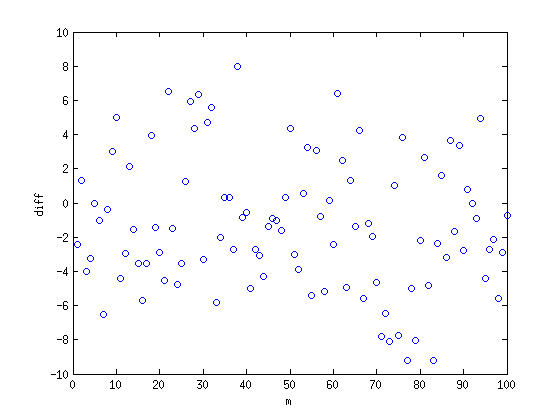
\includegraphics[width=\linewidth]{prob1_fig.png}

        \caption{\label{fig:prob1} Difference between $\bm{\hat{b}}$ and
        $\bm{b}_{\rm true}$ as a function of joke.}

    \end{figure} 

\end{homeworkProblem}
\clearpage
%===============================================================================

%===============================================================================
%-------------------------------------------------------------------------------
%	PROBLEM 2 
%-------------------------------------------------------------------------------
\begin{homeworkProblem}
    
    We perform the same method as in problem 1, except with the full
    100$\times$7,200 $\bm{A}$ data matrix. See Figure~\ref{fig:prob2} for the
    differences between our suggested ratings $\bm{\hat{b}}$ and the new user's
    true ratings, $\bm{b}_{\rm true}$. Our suggested highest rating for the
    user still does not match the true highest rating of the new user. The
    linear least squares solution is now underdetermined. The prediction is
    still not very good, there is a large scatter in the differences between
    the predicted ratings and the true ratings.

    \begin{figure}
        
        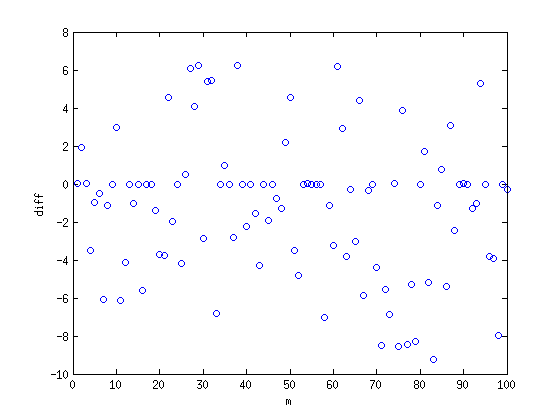
\includegraphics[width=\linewidth]{prob2_fig.png}

        \caption{\label{fig:prob2} Difference between $\bm{\hat{b}}$ and
        $\bm{b}_{\rm true}$ as a function of joke.}

    \end{figure}

\end{homeworkProblem}
\clearpage
%===============================================================================

%===============================================================================
%-------------------------------------------------------------------------------
%	PROBLEM 3
%-------------------------------------------------------------------------------
\begin{homeworkProblem}

    We can find the user with the closest ratings to the new user by
    calculating the square residuals between every previous user's ratings and
    the new user's ratings. The previous user with the smallest residual with
    the new user will be the most similar to the new user. We find that the
    closest user is 6528 and the second closest user is 2283 to the new user.

\end{homeworkProblem}
\clearpage
%===============================================================================

%===============================================================================
%-------------------------------------------------------------------------------
%	PROBLEM 4
%-------------------------------------------------------------------------------
\begin{homeworkProblem}

    The spectrum of $\bm{X}$ is shown in Figure~\ref{fig:prob4}. 4 dimensions
    seem to describe the dataset quite well. This means that there are four
    principal types of jokes, where if a user likes one of the four jokes, then
    we can make a reasonable prediction of which other jokes the user will like.
    The numerical rank of $\bm{X}$ is about 10. The flat slope of singular
    values means that there is noise in the data which the singular values are
    trying to explain.

    \begin{figure}[!ht]
        
        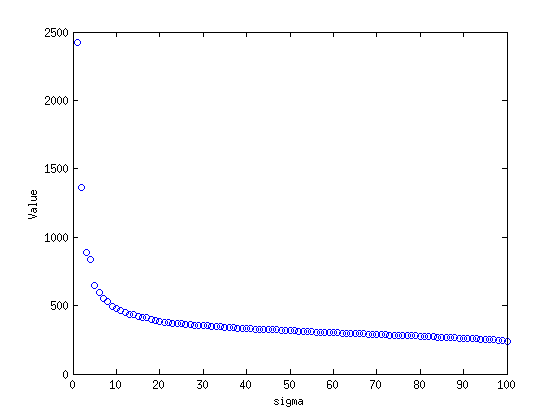
\includegraphics[width=\linewidth]{prob4_fig.png}

        \caption{\label{fig:prob4} Spectrum of SVD of $\bm{X}$. Four dimensions
        describe the dataset well.}

    \end{figure}

\end{homeworkProblem}
\clearpage
%===============================================================================

%===============================================================================
%-------------------------------------------------------------------------------
%	PROBLEM 5
%-------------------------------------------------------------------------------
\begin{homeworkProblem}
   
    Figure~\ref{fig:prob5} shows the columns and rows of $\bm{X}$ projected
    onto the first three principle component directions. 

    \begin{figure}[!ht]
        
        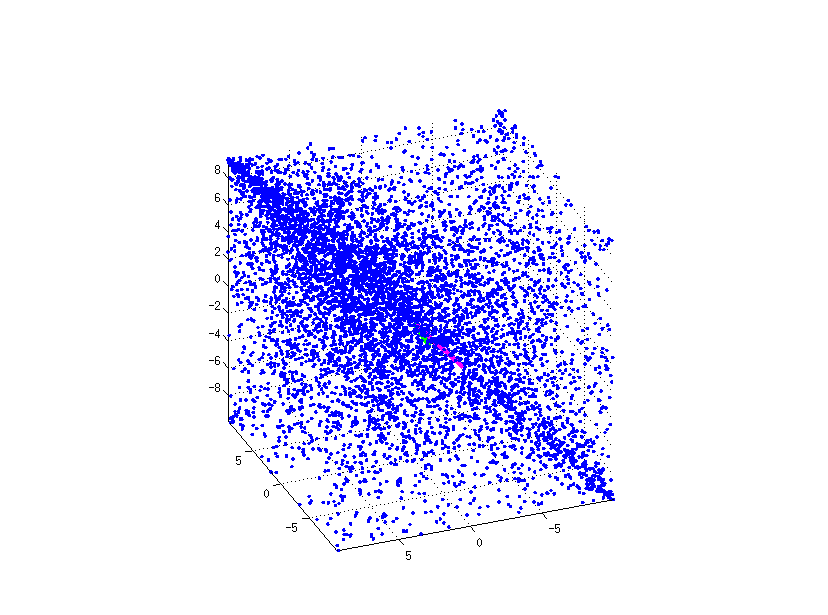
\includegraphics[width=\linewidth]{prob5_fig.png}

        \caption{\label{fig:prob5} Columns and rows of $\bm{X}$ projected onto
        the first three principle component directions. We can see that there
    is one dominant principle component which can describe the relationship
between jokes and users well.}

    \end{figure}


\end{homeworkProblem}
%===============================================================================

%===============================================================================
%-------------------------------------------------------------------------------
%	PROBLEM 6
%-------------------------------------------------------------------------------
\begin{homeworkProblem}
    
    The power iteration algorithm produces a single eigenvalue and eigenvector
    for a data matrix method A. First, the algorithm starts with either a guess
    for the dominant eigenvector or a random vector, $\bm{b_0}$. From there,
    the next vector $\bm{b}_k$ is found by 

    \begin{equation}
        \bm{b}_{k+1} = \frac{\bm{A}{b}_k}{\|\bm{A}\bm{b}_k\|}
    \end{equation}

    \noindent so that at each iteration the vector $\bm{b}_k$ is multiplied by
    the matrix $\bm{A}$ and normalized. The method does this until a subsequent
    eigenvector converges to an eigenvector associated with the dominant
    eigenvalue. This works only if $\bm{A}$ has an eigenvalue which is larger
    than its other eigenvalues. \\

    The 1-norm between 1st col of U and p is 16.4691 and the 1-norm between
    1st col of V and p is 13.8949. This tells us that there is a mild
    difference between the first principle component of the SVD and the
    eigenvector from the power method.

\end{homeworkProblem}
%===============================================================================

%===============================================================================
%-------------------------------------------------------------------------------
%	PROBLEM 7
%-------------------------------------------------------------------------------
\begin{homeworkProblem}

    A column vector of $m \times 1$ size of all zeros would break the power
    method, because the normalized eigenvector would immediately be in the null
    space of the data matrix.

\end{homeworkProblem}
\clearpage
%===============================================================================

Code:

Problem 1 \\
\pythonexternal{hw5_prob1.m} 
\clearpage

Problem 2 \\
\pythonexternal{hw5_prob2.m}
\clearpage

Problem 3 \\
\pythonexternal{hw5_prob3.m}
\clearpage

Problem 4 \\
\pythonexternal{hw5_prob4.m}
\clearpage

Problem 5 \\
\pythonexternal{hw5_prob5.m}
\clearpage

Problem 6 \\
\pythonexternal{hw5_prob6.m}
\pythonexternal{power_iter.m}

\end{document}

